\documentclass[11pt,a4paper]{article}
\usepackage[margin=2.5cm]{geometry}
\usepackage{listings}
\usepackage{xcolor}
\usepackage{graphicx}
\usepackage{booktabs}
\usepackage{amsmath}
\usepackage{hyperref}
\usepackage{parskip}

\lstset{
    language=C,
    basicstyle=\ttfamily\small,
    keywordstyle=\color{blue}\bfseries,
    commentstyle=\color{gray},
    stringstyle=\color{orange},
    frame=single,
    breaklines=true,
    numbers=left,
    numberstyle=\tiny\color{gray}
}

\title{\textbf{TP5: MPI Point-to-Point and Collective Communications}}
\author{Khaoula Mejhoudi}
\date{February 2025}

\begin{document}
\maketitle

% -------------------------------------------------------
\section{Exercise 1: Hello World}

The goal was to write a basic MPI program. Each process prints its rank and the total number of processes. Only rank 0 prints an extra message.

\begin{lstlisting}
MPI_Comm_size(MPI_COMM_WORLD, &size);
MPI_Comm_rank(MPI_COMM_WORLD, &rank);
printf("I am process %d among %d\n", rank, size);
if (rank == 0) printf("I'm here alone\n");
\end{lstlisting}

Omitting \texttt{MPI\_Finalize()} causes MPI resources to not be released properly. In practice, most implementations still terminate, but it is undefined behavior and can cause issues in some environments.

% -------------------------------------------------------
\section{Exercise 2: Sharing Data}

Process 0 reads an integer and broadcasts it to all processes using \texttt{MPI\_Bcast}. This repeats until a negative value is entered.

\texttt{MPI\_Bcast} is a collective operation: every process must call it, but only the root (rank 0) provides the data. All others receive it.

\begin{lstlisting}
do {
    if (rank == 0) scanf("%d", &v);
    MPI_Bcast(&v, 1, MPI_INT, 0, MPI_COMM_WORLD);
    printf("Process %d received %d\n", rank, v);
} while (v >= 0);
\end{lstlisting}

% -------------------------------------------------------
\section{Exercise 3: Sending in a Ring}

Process 0 reads a value, sends it to process 1. Each process receives the value, adds its rank, prints the result, and forwards it to the next process.

The communication pattern uses only \texttt{MPI\_Send} and \texttt{MPI\_Recv}:
\begin{itemize}
    \item Process 0: reads, sends to rank+1 (no receive).
    \item Middle processes: receive from rank$-1$, add rank, print, send to rank+1.
    \item Last process: receives, adds rank, prints (no send).
\end{itemize}

Process 0 sends before any receive happens, which prevents deadlock since the ring flows in one direction.

% -------------------------------------------------------
\section{Exercise 4: Matrix-Vector Product}

\subsection{Implementation}

The matrix $A$ (size $N \times N$) is distributed row-by-row across processes using \texttt{MPI\_Scatterv}. The vector $b$ is sent to all processes using \texttt{MPI\_Bcast}. Each process computes its portion of the result, and results are collected with \texttt{MPI\_Gatherv}.

\texttt{MPI\_Scatterv} (instead of \texttt{MPI\_Scatter}) is used to handle cases where $N$ is not divisible by the number of processes. The first $N \mod P$ processes get one extra row.

The parallel workflow is:
\[
\text{Bcast}(b) \;\rightarrow\; \text{Scatterv}(A) \;\rightarrow\; \text{local multiply} \;\rightarrow\; \text{Gatherv}(x)
\]

\subsection{Results}

\begin{table}[h]
\centering
\begin{tabular}{cccccc}
\toprule
$N$ & $P=1$ (s) & $P=2$ (s) & $P=4$ (s) & $P=8$ (s) & Speedup ($P=4$) \\
\midrule
1000  & 0.0074 & 0.0067 & 0.0071 & 0.0213 & 1.04 \\
4000  & 0.1250 & 0.1203 & 0.1247 & 0.2030 & 1.00 \\
8000  & 0.5170 & 0.5142 & 0.5036 & 0.5537 & 1.03 \\
10000 & 0.7949 & 0.7403 & 0.8033 & 0.8779 & 0.99 \\
\bottomrule
\end{tabular}
\caption{Execution times for matrix-vector multiplication}
\end{table}

\begin{figure}[h]
    \centering
    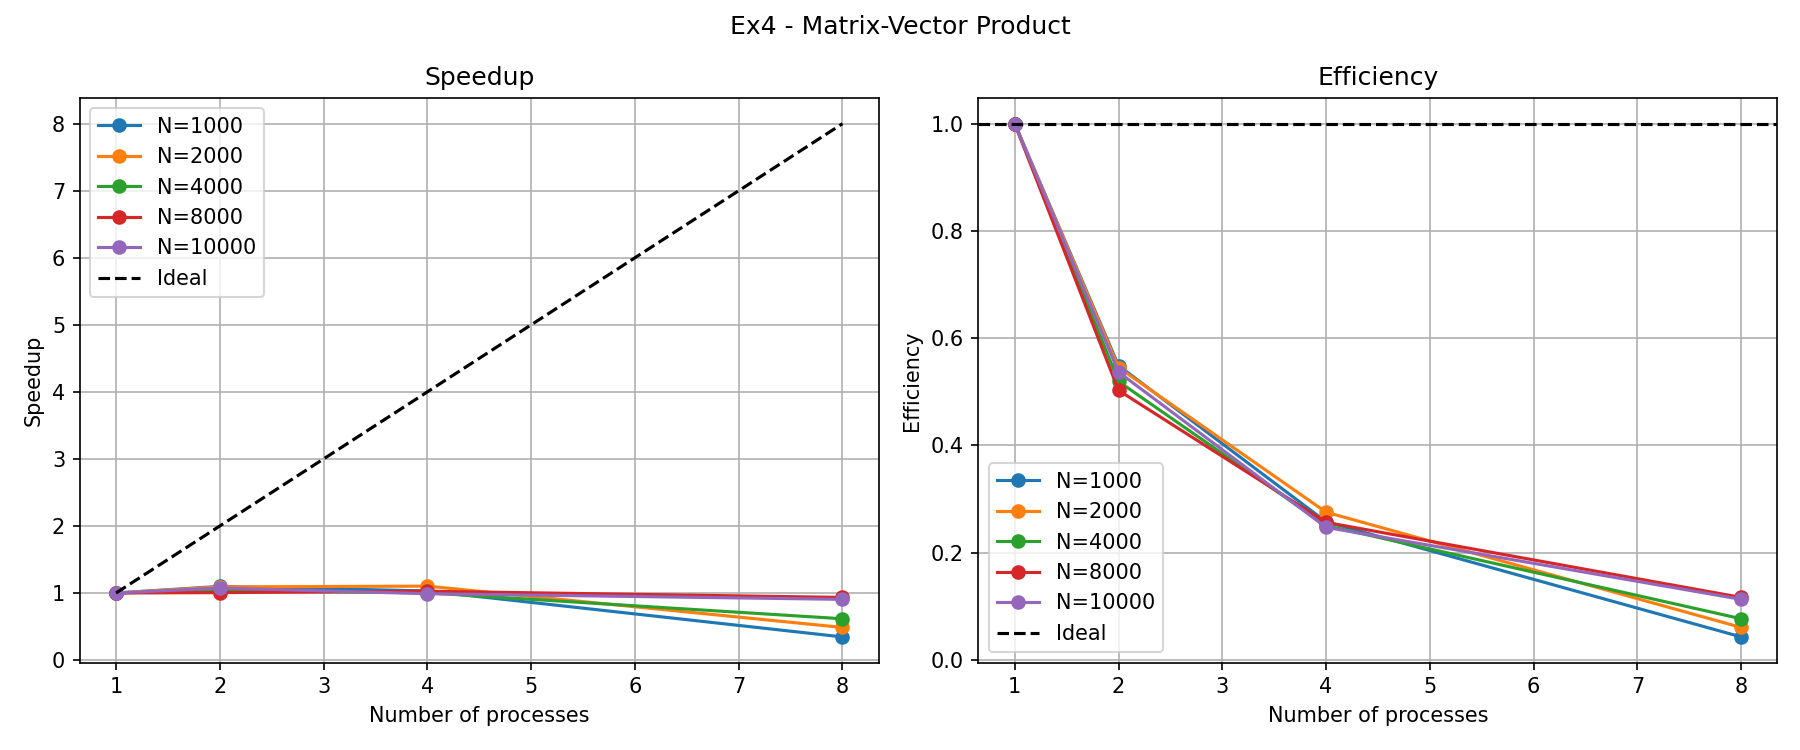
\includegraphics[width=0.9\textwidth]{speedup_ex4.png}
    \caption{Speedup and Efficiency: Matrix-Vector Product}
\end{figure}

\subsection{Analysis}

The speedup is very close to 1 regardless of the number of processes. This is expected: the bottleneck is communication, not computation. \texttt{MPI\_Scatterv} must send $O(N^2)$ data to each process, which is the same cost as the computation itself. The communication overhead cancels out any gain from parallelism. With 8 processes the program is even slower due to synchronization overhead.

For this type of problem, MPI parallelism only becomes worthwhile at very large $N$ where computation time dominates communication time.

% -------------------------------------------------------
\section{Exercise 5: Pi Calculation}

\subsection{Implementation}

$\pi$ is approximated using:
\[
\pi \approx \frac{4}{N} \sum_{i=0}^{N-1} \frac{1}{1 + x_i^2}, \quad x_i = \frac{i + 0.5}{N}
\]

Each process handles every $P$-th iteration (interleaved distribution): process $r$ computes $i = r, r+P, r+2P, \ldots$ This naturally handles cases where $N$ is not divisible by $P$ without any special logic.

Each process computes a local partial sum. \texttt{MPI\_Reduce} with \texttt{MPI\_SUM} collects all partial sums into the final result on rank 0.

\subsection{Results}

\begin{table}[h]
\centering
\begin{tabular}{cccccc}
\toprule
$N$ & $P=1$ (s) & $P=2$ (s) & $P=4$ (s) & $P=8$ (s) & Speedup ($P=4$) \\
\midrule
$10^6$  & 0.0037 & 0.0019 & 0.0011 & 0.0013 & 3.51 \\
$10^7$  & 0.0331 & 0.0181 & 0.0088 & 0.0094 & 3.76 \\
$10^8$  & 0.3436 & 0.1716 & 0.1090 & 0.1096 & 3.15 \\
$10^9$  & 3.4725 & 1.7525 & 0.8823 & 1.0839 & 3.94 \\
\bottomrule
\end{tabular}
\caption{Execution times for Pi calculation}
\end{table}

\begin{figure}[h]
    \centering
    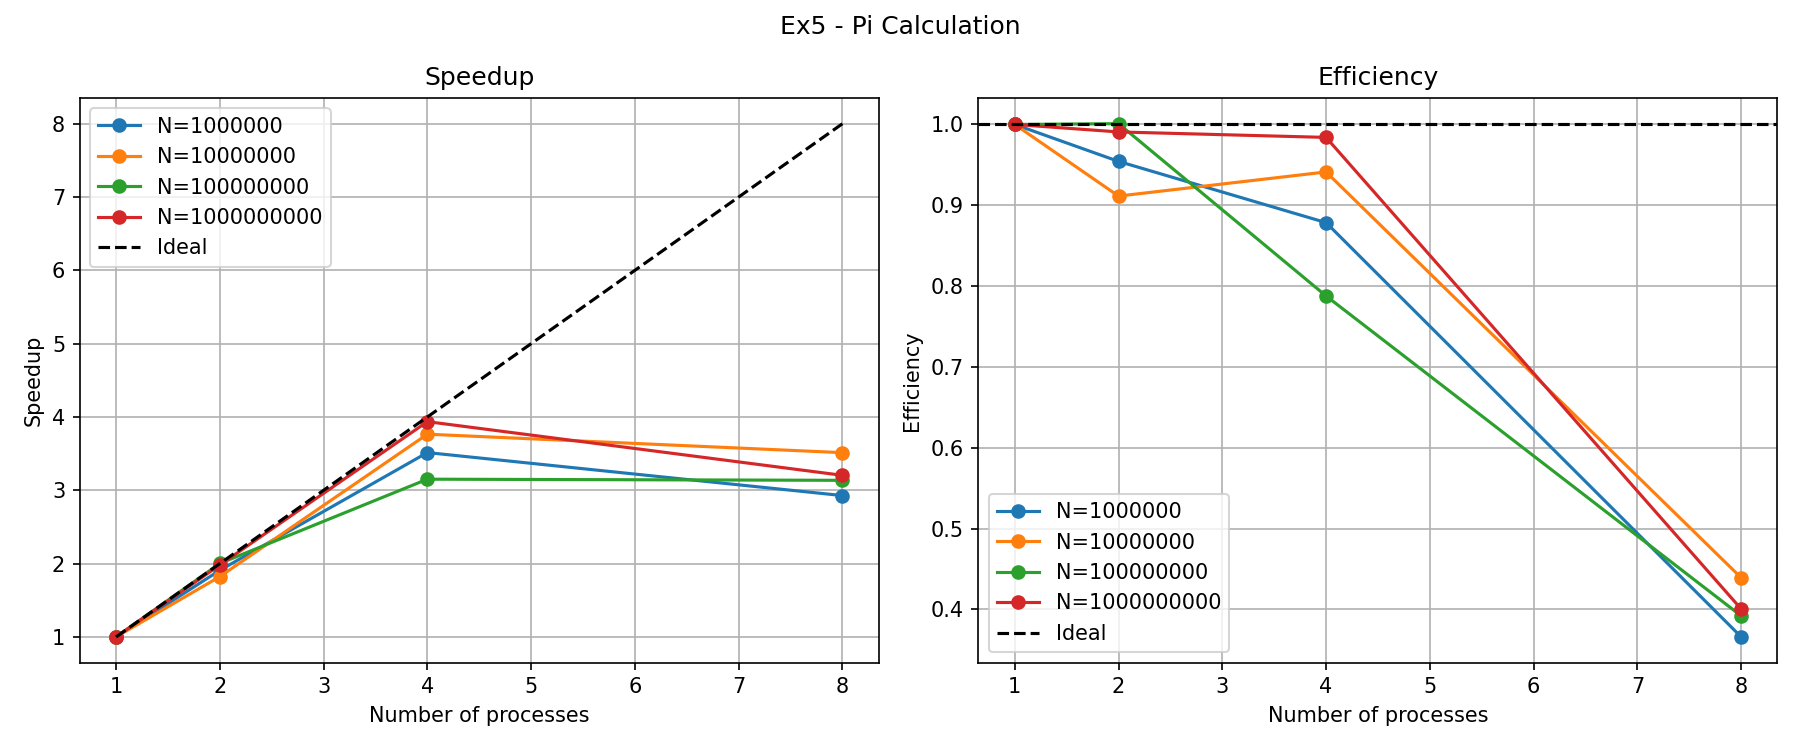
\includegraphics[width=0.9\textwidth]{speedup_ex5.png}
    \caption{Speedup and Efficiency: Pi Calculation}
\end{figure}

\subsection{Analysis}

Pi calculation shows near-linear speedup with 4 processes (speedup $\approx 3.94$ for $N=10^9$, efficiency $\approx 98\%$). This is because each iteration is independent and the only communication is a single \texttt{MPI\_Reduce} call at the end, so the communication cost is $O(1)$ regardless of $N$.

With 8 processes, performance drops slightly compared to 4 (speedup $\approx 3.20$). On this cluster, the benefit of 8 processes is limited likely due to shared resources or NUMA effects on the login node.

This exercise illustrates a perfectly parallel workload: no data dependencies, minimal communication. It is a good example of Amdahl's law: since there is almost no sequential part, the speedup scales nearly linearly with the number of processes.

% -------------------------------------------------------
\section{Conclusion}

This lab covered the two main types of MPI communication:

\begin{itemize}
    \item \textbf{Point-to-point} (\texttt{MPI\_Send}/\texttt{MPI\_Recv}): used in the ring exercise. Simple but requires careful ordering to avoid deadlock.
    \item \textbf{Collective} (\texttt{MPI\_Bcast}, \texttt{MPI\_Scatter}/\texttt{Gather}, \texttt{MPI\_Reduce}): used in exercises 2, 4, and 5. More expressive and often better optimized by the MPI library.
\end{itemize}

The key lesson from the performance results is that \textbf{communication overhead matters}. Pi calculation parallelizes well because communication is minimal ($O(1)$). Matrix-vector multiplication does not scale here because the cost of distributing the matrix ($O(N^2)$) equals the computation cost, leaving no room for speedup.

\end{document}
